\chapter{GPU Computing}

\section{OpenGL}
OpenGL is a cross-platform and open industry standard for programming two and
three dimensional graphics.\cite{OpenGL} The most common use of OpenGL is for programming on
dedicated graphics hardware. OpenGL is supported by all of the major graphics
cards makers, operating systems and game development studios.


Dedicated graphics hardware is generally a combination of special processors
and memory designed for the kind of vector processing commonly encountered in
graphics programming. One of the primary tasks in graphics programming is
rasterization. Rasterization is the process of representing a three-dimensional
scene as a set of discrete, two-dimensional pixels. While there are various
techniques for rasterization, an underlying theme is the necessity for a large
amount of independent calculations being done for each pixel. These operations
include many linear algebra and other floating point math operations useful for
two and three-dimensional geometry and effects.\cite{Luebke2007}


As graphics hardware became more sophisticated, more control of this parallel
infrastructure has been given to the programmer. This became popular with the
advent of $shaders$, small programs which could be executed by the graphics
hardware to do more sophisticated computational operations than available
through the standard interface. Shaders were named for their primary use of
shading and lighting objects, which often times calls for the computation of
sophisticated mathematical and physical models. OpenGL provides a programming
language called GLSL for writing shaders, which allows the programmer to
manipulate vertices, colors, textures, and recently geometry all in parallel.\cite{Luebke2007}


\section{General Purpose GPU Programming}


With the advances in graphics hardware, most notably with the introduction of
shaders, the GPU began to share similarities with the vector processing
architectures used in supercomputers for scientific simulations. Researchers
began using GPUs to compute problems suitable for a parallel vector processor
at a fraction of the cost of a super computer. The speed benefits of using a
GPU over a CPU for highly parallel problems at a low cost has generated
increasing interest in using the GPU for general purpose computing.\cite{Owens2007}


\section{GPU Programming Languages}

Programming languages available for programming GPUs have evolved over the last
decade from specialized graphics languages into general purpose programming
languages such as CUDA and OpenCL.\cite{Owens2007}

\begin{figure}[!htc]
 		\centering
		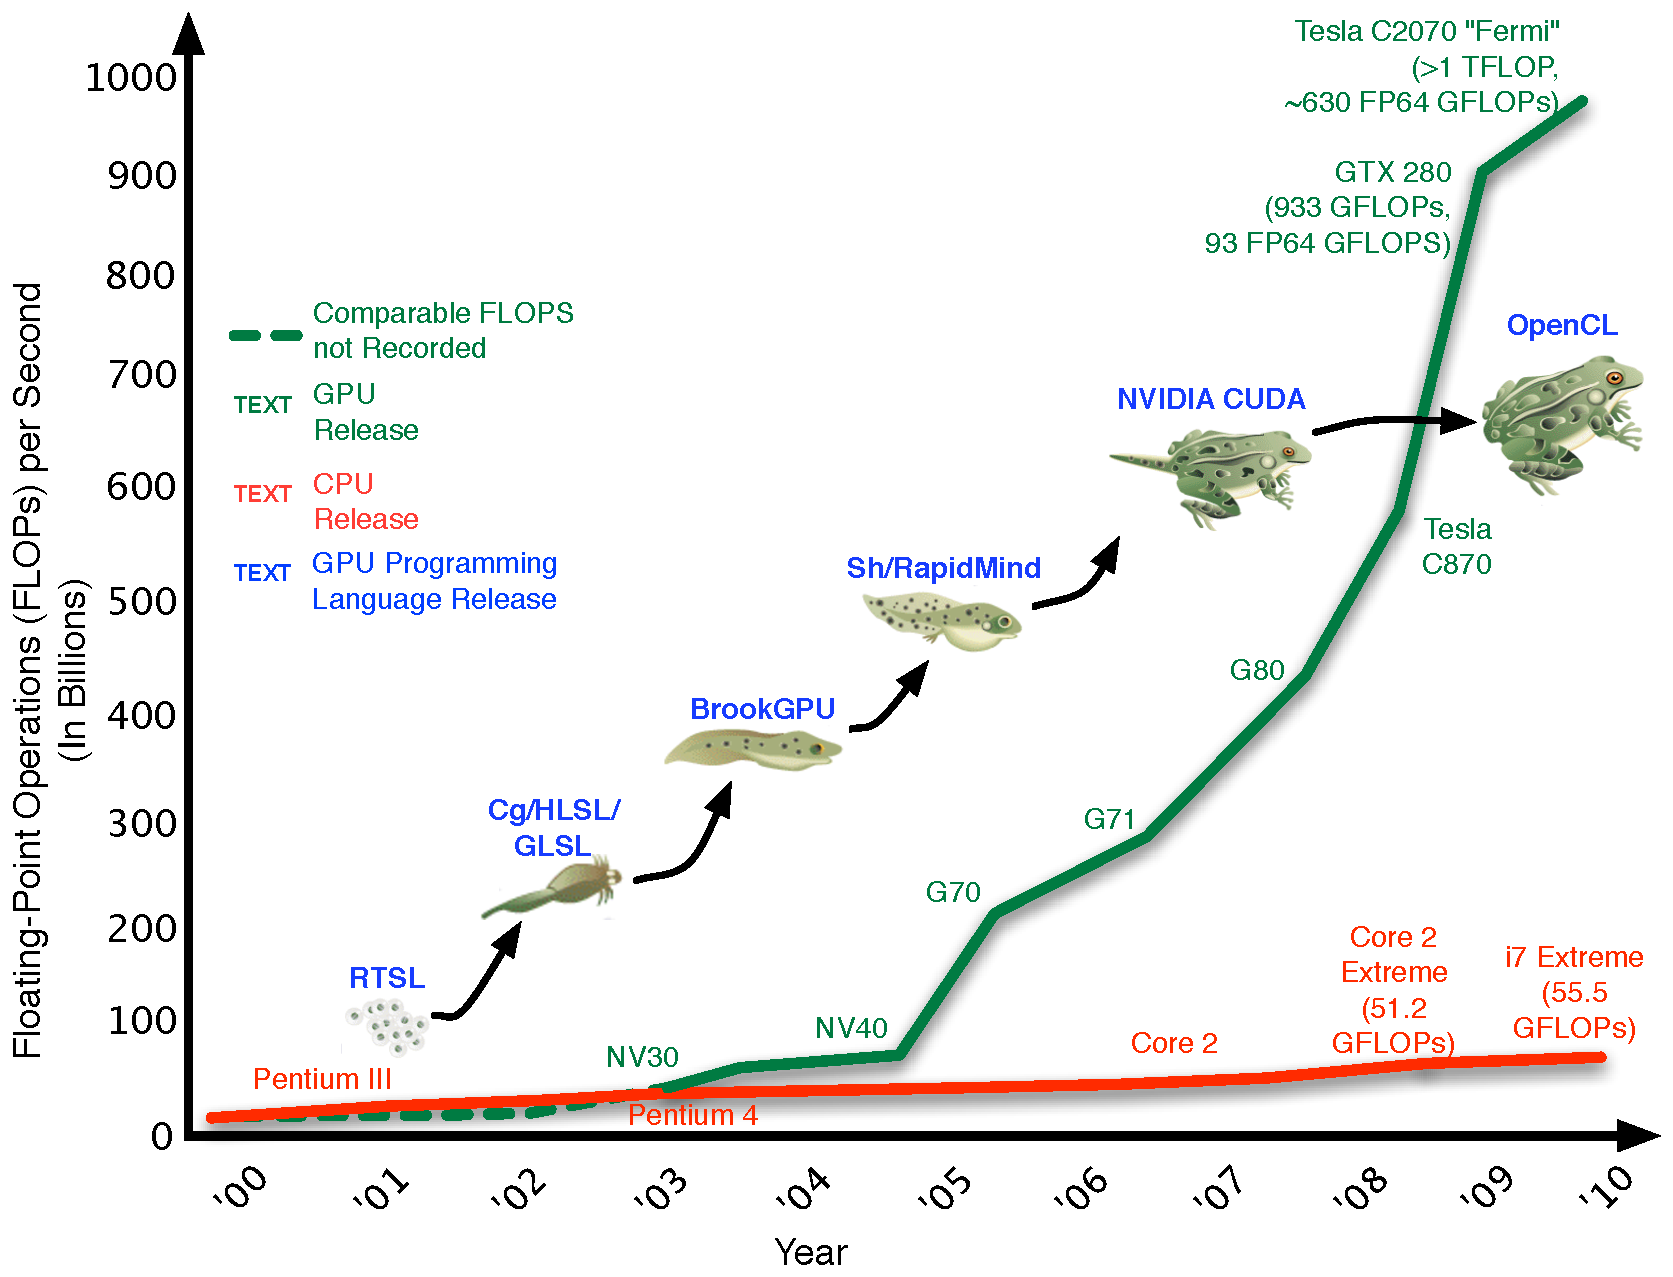
\includegraphics[scale=.55]{figures/GPU_Evolution_opencl.pdf}
		%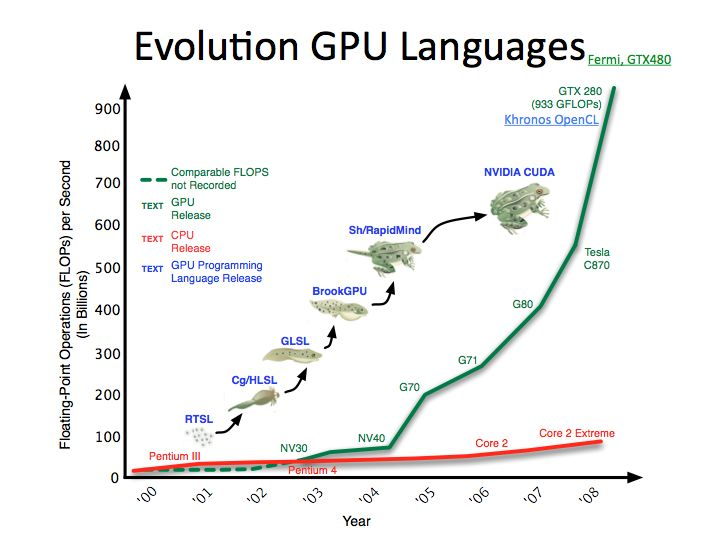
\includegraphics[scale=.6]{figures/frogs.jpg}
        \caption{ GPU Programming Language Evolution \cite{Bollig} }
        \label{fig:frogs}
\end{figure}



\subsection{CUDA}
In 2006 graphics card manufacturer NVIDIA created the CUDA architecture 
for general purpose computing on NVIDIA GPUs. CUDA is programmed with the 'C
for CUDA' language, which abstracts access to the GPU resources. CUDA provides
familiar programming techniques such as template programming and memory access
and manipulation with pointers. CUDA is leading the GPGPU market in performance
and features, however due to its proprietary nature and lack of availability on
competing platforms such as AMD or Intel it was not considered as an option for
this project.


\subsection{OpenCL}

In 2009 OpenCL was released as an open standard for a parallel computing
language and runtime API by Khronos, an industry run consortium which also
controls the OpenGL standard.\cite{OpenCL} The OpenCL specification provides
for two things, the OpenCL runtime and the OpenCL programming language. The
OpenCL runtime is designed for parallel programming in heterogeneous
environments, providing mechanisms for dealing with multiple and varied compute
devices such as CPUs and the many types and generations of GPUs.  The OpenCL
programming language is a derivative of C99, giving it familiar syntax in an
otherwise unfamiliar context for many programmers.


OpenCL is more recent and less mature of a language than CUDA, additionally it
is designed by a consortium rather than a single company so innovation is
adopted rather than pushed. OpenCL still lacks several features such as
templates and memory addressing which make programming easier. The fact that it
is an open standard supported by the largest entities in the computing industry
are the motivation behind choosing a less featureful environment for this
project. It is expected that OpenCL will continue to improve for some time and
is a relatively safe bet for institutions with long-term plans.



\section{Architecture}
The idea behind the architecture of a Graphics Processing Unit is to have many
smaller floating point processors operate on a large amount of data in
parallel.
The way this is achieved in general is by implementing a memory hierarchy which
allows each processor to quickly operate on data which it needs. The OpenCL 
memory model is given in Figure \ref{fig:gpu_memory}

\begin{figure}[!htc]
 		\centering
		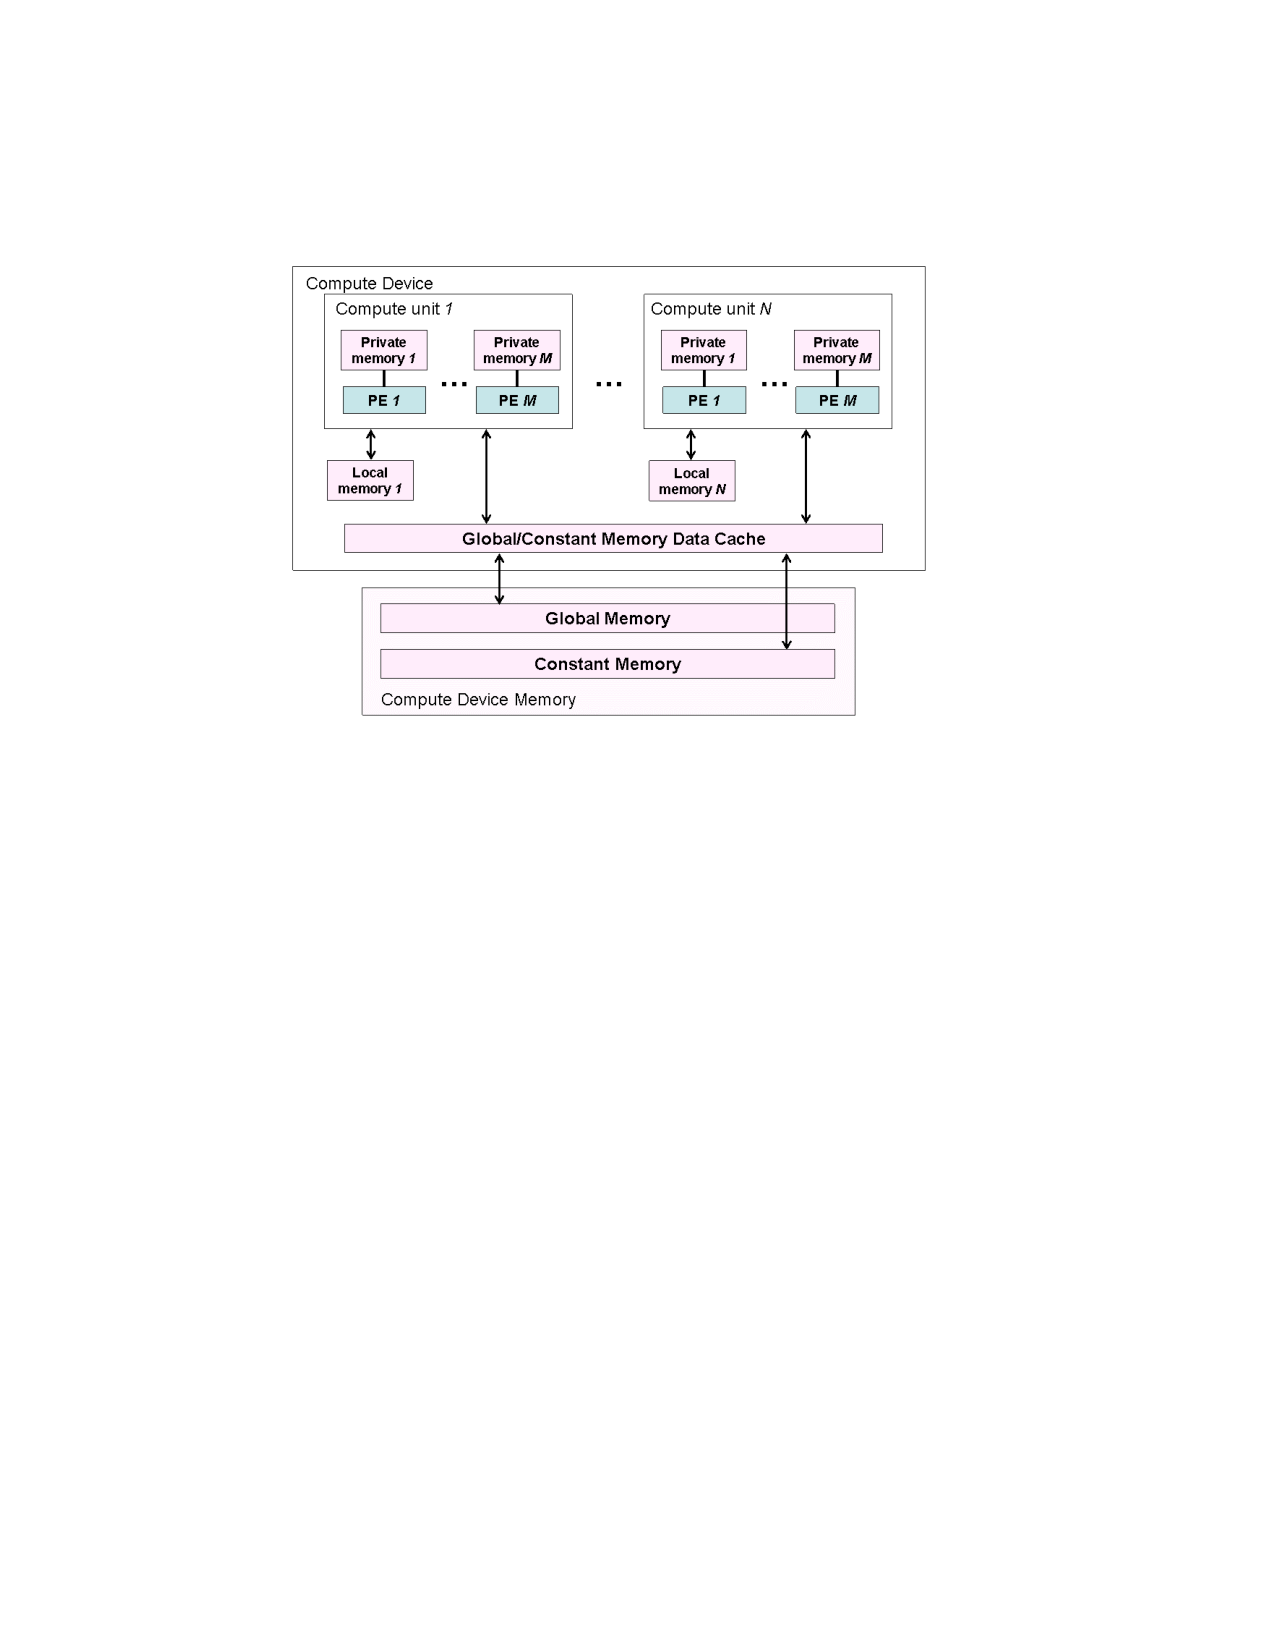
\includegraphics[scale=1.0]{figures/gpu_memory.pdf}
        \caption{ OpenCL Memory Hierarchy Diagram \cite{OpenCLSpec} }
        \label{fig:gpu_memory}
\end{figure}

The figure shows four main types of memory: $global$, $constant$, $local$ and
$private$. $Global$ memory is memory available to all of the processors (known
as compute units) and is the slowest type of memory in the hierarchy.
$Constant$ memory is memory which is read-only by the compute units, and is
usually cached for fast access. $Local$ memory is specific to each compute
unit, while much faster than $global$ memory it cannot be used to communicate
between compute units. Compute units are further divided into workers, which
can be thought of as individual threads which each have their own $private$
memory. Threads are executed in batches called work-groups, and each thread in a
work-group has access to the same bank of $local$ memory, as well as access to
all of the $global$ memory. 


Threads, or work items, in a work-group are executed simultaneously and in
parallel, unless the kernel being executed contains $branching$ code such as if
statements. In the event of branching threads for each branch will execute
synchronously, limiting the effectiveness of the GPU. Since $local$ memory
access is normally at least an order of magnitude faster than $global$ memory
access, $local$ memory is often used as a user controlled cache. A common
technique is to copy frequently used $global$ memory to $local$ memory with one
thread, synchronizing the threads with a barrier and then processing the
$local$ memory in parallel. 


$Local$ and $global$ memory are consistent at a work-group barrier, meaning all
threads will see the same value in memory after a barrier is placed. $Global$
memory is not guaranteed to be consistent across work-groups so it is important
to avoid memory conflicts within a single kernel launch.

\subsection{OpenCL Runtime}

In order to execute programs written in OpenCL a programmer must first use the
OpenCL runtime API to setup a $context$. An OpenCL context provides the
programmer with resources available from $devices$ within that context (such as
a GPU). The programmer may send memory as well as programs to the context
through the use of a $command queue$. Commands in the command queue may be
executed synchronously or asynchronously at the programmers behest. The most
important items manipulated in the command queue are $kernels$ and $buffers$.
Kernels are the OpenCL programs which will be executed on a particular device
while buffers are the memory which the kernels can take as arguments (i.e.
arrays). Kernels are compiled at runtime by OpenCL, allowing the same code to
be run on different device architectures without any guidance from the
programmer.



